\documentclass[portrait,a0paper,fontscale=0.277]{baposter}

\usepackage{enumitem}
\setlist{nolistsep}

%\usepackage[spanish]{babel}
\usepackage[utf8]{inputenc}
\usepackage{graphicx}
\usepackage{wrapfig}
%\usepackage{capt-of}
\usepackage{captdef}

\usepackage{tikz}
\usetikzlibrary{calc,automata,positioning,arrows}

\tikzstyle{line} = [draw, -latex]

%%%%%%%%%%%%%%%%%%%%%%%%%%%%%%%%%%%%%%%%%%%%%%%%%%%%%%%%%%%%%%%%%%%%%%%%%%%%%%%%
% Save space in lists. Use this after the opening of the list
%%%%%%%%%%%%%%%%%%%%%%%%%%%%%%%%%%%%%%%%%%%%%%%%%%%%%%%%%%%%%%%%%%%%%%%%%%%%%%%%
\newcommand{\compresslist}{%
\setlength{\topsep}{0pt}%
\setlength{\itemsep}{0pt}%
\setlength{\parskip}{0pt}%
\setlength{\parsep}{0pt}%
}

\begin{document}
\begin{poster}
{ 
	background=plain,
	bgColorOne=white,
	borderColor=orange,
	linewidth=2pt,
	headershade=plain,
	headerColorOne=orange,
	boxshade=plain,
	boxColorOne=white,
	boxColorTwo=orange,
	textborder=roundedsmall,
	headerborder=open,
	headershape=smallrounded,
	headerheight=0.07\textheight,
	headerfont=\large\bf\textsc, %Sans Serif
	eyecatcher=true
}
{ \includegraphics[height=5.0em]{eji_logo} }
{ \Large\bf\textsc{7.7.1 Localización de Manos por Webcam  aplicado a Interfaz para Dibujo} }
{ \textsc\small{ \large{Bedrij Walter, Benitez Federico, Benitez Fernado} \\ \footnotesize {wbedrij@gmail.com, federicobenitez2@gmail.com, fernandobenitezfich@gmail.com} } }  { \includegraphics[height=5.0em]{fich2} }

	\headerbox{Introducción}{name=intro,column=0,row=0}{
	
	Objetivos:
	\begin{itemize}\compresslist	
	\item Desarrollar un algoritmo que permita localizar la posición de las manos.
	\item Describir su trayectoria teniendo como entrada un vídeo sacado de una cámara web.
	\item Crear interfaces aéreas sin la utilización de marcadores.
	\item Localizar las manos en tiempo real.
	\end{itemize}

	Alcance: 
	\begin{itemize}\compresslist	
	\item No se aborda el seguimiento de la mano.  
	\item No se aborda la resolución de casos en donde la mano se encuentra sobre la cara.
	\item Se supone  el brazo cubierto. 
	\end{itemize}
	}

\headerbox{Imágenes de Interés }{name=ana,column=1,span=2,row=0}{
	\begin{center}
	\begin{tabular}{ccc}
		\includegraphics[width=.28\textwidth]{fondo.png} &
		\includegraphics[width=.28\textwidth]{hue.png} &
		\includegraphics[width=.28\textwidth]{fondoandhue.png} \\

		Fondo & Hue & Fondo AND Hue \\
	\end{tabular}
	\end{center}
	\begin{center}
	\begin{tabular}{cc}
		\includegraphics[width=.28\textwidth]{final.png} &
		\includegraphics[width=.28\textwidth]{interfaz.png} \\

		Objeto Ganador & Interfaz \\
	\end{tabular}
	\end{center}
}
	\headerbox{Metodología}{name=nn,column=1,span=2,below=ana}{

	\begin{center}
	\begin{tabular}{c}
		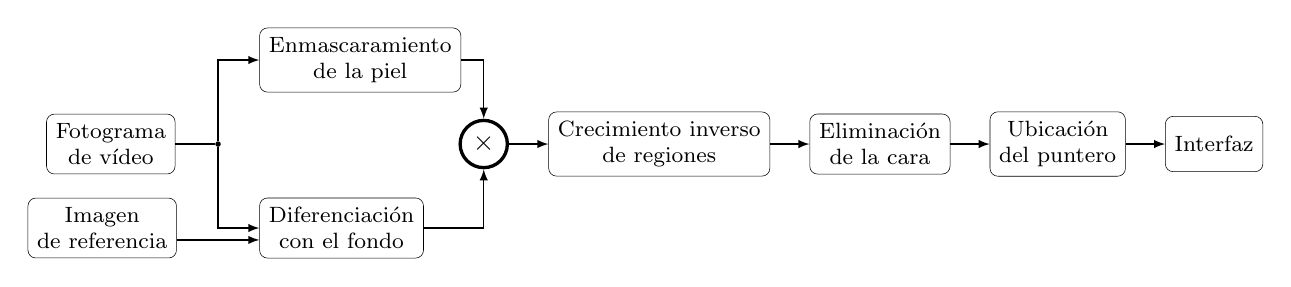
\begin{tikzpicture}[
	%scale=0.6,
	every node/.style={transform shape},
	node distance=10mm and 5mm,
	nonterminal/.style={
		rectangle,
		rounded corners=3mm,
		minimum size=6mm,
		very thick,
		draw=black,
	},
	terminal/.style={
		rectangle,
		minimum size=2em,
		rounded corners=1mm,
		very thin,
		draw=black,
		font=\footnotesize,
		%text width=15ex,
		align=center,
		%text centered
	},
	point/.style={
		circle,
		inner sep=0pt,
	}
]
	\node (start) [terminal]
		{Fotograma \\de vídeo};
	\node (p0) [point,minimum size=2pt,fill=black,right=of start] {};
	\node (p1) [point,above=of p0] {};
	\node (p2) [point,below=of p0] {};
	\node (skin) [terminal,right=of p1]
		{Enmascaramiento \\de la piel};
	\node (p3) [point,right=of skin] {};
	\node (diff) [terminal,right=of p2]
		{Diferenciación \\con el fondo};
	\node (ref) [terminal,left=of p2]
		{Imagen \\de referencia};
	\node (p4) [point,right=of diff] {};
	%\node (p5) [point,above=of p4] {};
	\node (and) [nonterminal] at ($(p3) !.5! (p4)$)
		{$\times$};
	\node (growth) [terminal,right=of and]
		{Crecimiento inverso \\de regiones};
	\node (face) [terminal,right=of growth]
		{Eliminación \\de la cara};
	\node (pointer) [terminal,right=of face]
		{Ubicación \\del puntero};
	\node (interfaz) [terminal,right=of pointer]
		{Interfaz};

	\draw  (start) -- (p0);
	\draw [line] (p0) |- (skin);
	\draw [line] (p0) |- (diff);
	\draw [line] ([yshift=-1ex]ref.east) -- ([yshift=-1ex]diff.west);
	\draw [line] (skin) -| (and);
	\draw [line] (diff) -| (and);
	\draw [line] (and) -- (growth);
	\draw [line] (growth) -- (face);
	\draw [line] (face) -- (pointer);
	\draw [line] (pointer) -- (interfaz);


\end{tikzpicture}
 \\
		%\includegraphics[width=\textwidth-2em]{diagrama.pdf} \\
		Diagrama en bloques
	\end{tabular}
	\end{center}

	\begin{description}
		\item[Diferenciación con el fondo] \hfill
		\begin{itemize}\compresslist
			\item Se realiza la diferencia entre los canales RGB del frame actual contra la imagen de referencia del fondo. Esto permite discriminar al objeto.
		\end{itemize}
		\item[Enmascaramiento de la piel] \hfill
			\begin{itemize}\compresslist
			\item Se usó  la información del  Hue,  como  sugiere  [2]. 
			\item Como  pre-proceso se aplica un filtro de mediana,  tratando  además  de  uniformar  la
			textura de la piel. 
			\item Se aplica un umbral global en la  componente  $H$  dejando pasar el rango $H = 14 \pm 10$ (valores experimentales de la piel).

			\item Para eliminar los huecos internos en el Hue, 
			%\begin{itemize}\compresslist
			%\item
 se procedió  aplicar  un  cierre morfológico con un elemento estructurante de forma cuadrada y tamaño de  $5 \times 5$,como se explica en [1].
			%\end{itemize}
			\item Al resultado, se aplica un AND con la máscara de diferencia, obteniéndose objetos  no
			pertenecientes al fondo con un tono parecido al de la piel.
			\end{itemize}


		\item[Crecimiento inverso de regiones] \hfill

			\begin{itemize}\compresslist	
			 \item Otro método  para  eliminar  los  huecos, como se observa en [3].
				%\begin{itemize}\compresslist	
					Sobre el Hue, a partir de  un  punto  que  se conoce fuera de cualquier zona de  interés,  realizamos  el  crecimiento  de
					regiones. 
					%\item 
\item Con esto obtenemos el fondo, al invertir  la  máscara  se tendrán
					las siluetas de los objetos.
				%\end{itemize}
			\end{itemize}	
		\item[Eliminación de la cara] \hfill
			\begin{itemize}\compresslist	
			\item Luego del proceso anterior, se tiene una imagen compuesta por  objetos  tipo
			piel. Se etiquetan las  regiones, quedándose con las 3  de  mayor
			área.
			\item Si resulta que  alguna  es  excesivamente
			pequeña con respecto a  las  otras  ($25 \%$)  es  considerada  como  ruido  y
			eliminada.

			\item Queda  eliminar la región que identifica a la cara. Para facilitar el proceso, la mano debe
			tener un dedo extendido: 
			\begin{itemize}\compresslist
			\item Suponiendo a la cara como redonda, es de esperar
			que al hacer el factor de  redondez
			\[ C = \frac{\makebox{Área}}{\pi r^2}\]
			sea cercano a 1, quedando así la cara diferenciada de las manos. Donde $r$  es
			el radio del círculo cuyo centro se corresponde al centroide de la región  y
			pasa por su punto más alejado.% , dicho punto es  elegido como puntero de la región de interez.
			\end{itemize}
			\end{itemize}
		\item[Ubicación del puntero] \hfill
		\begin{itemize}\compresslist
		\item De las áreas interesantes obtenidas se designa como puntero el punto de la región  más lejano de su centroide .
		\end{itemize}
	
	\end{description}
	}

\headerbox{Resultados}{name=resultados,column=0,below=intro}{
		\begin{itemize}\compresslist
		\item El uso de una imagen de referencia permitió  que  la  mano  se
		ubicara sobre zonas de tonalidad parecida.

		\item El  Hue  mostró  ser  bastante  robusto  a  los  cambios  de  intensidad  de
		iluminación.

		\item Cuando se captó el dedo como  una  región  separada de la palma, fue
		eliminado por su  área  insignificante,  quedando   la  palma  de  forma
		aproximadamente circular, fallando así la heurística .

		\item Se observó oscilaciones  instantáneas de los punteros 
		producto de detecciones de  puntos  lejanos  no  deseados. \\
		En los Casos: 
			\begin{itemize}\compresslist
			\item Cuando se tenía el brazo descubierto
			\item Cuando se fragmentaba la región del dedo
			\end{itemize}

		\end{itemize}
	}
  \headerbox{Conclusión y Futuro Trabajo}{name=questions,below=resultados}{
		\begin{itemize}\compresslist
		\item La detección de la posición de las manos fue posible en tiempo real.

		\item Se necesitó usar una conformación en las posiciones de los dedos. 

		\item Problemas en la segmentación generaba falsas identificaciones, permitiendo
		 discontinuidades en las posiciones de los punteros.

		\item Para intentar solventar esos problemas se propone:
			\begin{itemize}\compresslist	
				 \item Realizar tracking de las manos, requiriendo una detección global inicial.
				 \item Realizar un refinamiento en la selección del punto característico.
	  		\end{itemize}
		\end{itemize}
  }



  \headerbox{Referencias}{name=referencias,column=0,above=bottom}{
%%%%%%%%%%%%%%%%%%%%%%%%%%%%%%%%%%%%%%%%%%%%%%%%%%%%%%%%%%%%%%%%%%%%%%%%%%%%%%
    \bibliographystyle{ieee}
    \renewcommand{\section}[2]{\vskip 0.05em}
      \begin{thebibliography}{1}\itemsep=-0.01em
      \setlength{\baselineskip}{0.4em}
	  \bibitem{gonzales2002:manual}
	  	Rafael Gonzales, Richard Woods.
		\newblock{Digital Image Processing.}
		\newblock{Prentice Hall.}
		\newblock{Estados Unidos, 2002.}
      \bibitem{chenk:hue}
      		\newblock{H. D. Cheng, X. H. Jiang, Y. Sun, y J. L. Wang. Color image segmentation: Advances \& prospects. Pattern Recognition, vol. 34, pp. 2259–2281. Estados Unidos, 2001.}
      \bibitem{pablo:fondo}
		\newblock{Javier Godoy, Pablo Novara  y Juan Vogt. Reconocimiento de señas. 37 Jornadas Argentinas de Informática e Investigación Operativa. Argentina, 2008.}
      \end{thebibliography}
   %\vspace{0.3em}
  }

\end{poster}
\end{document}
